\chapter{Basic Datastructures}

% the problem of working with individual values

\section{Types}

\subsection{Complex Types}

\subsection{Reference Types}

\section{Sequences in Data}

\subsection{Arrays}

\subsubsection{Indexing}

% calculation, this is why most languages agree that arrays start at zero

\subsubsection{Multidimensiontal Arrays}

\subsection{Linked Lists}

% head and tail

\subsection{Doubly Linked Lists}

\subsection{Looping Sequences}

\subsection{Nesting}

\section{Structured Data}

\subsection{Colors}

% light as a spectrum
Light is made up of photons, and each photon has a wavelength. The wavelength of the photons determines which color our eyes will observe. A wavelength of 380nm is violet and one of 740nm is red. In between these you have all the colors of the rainbow, in the order of the rainbow. Coincidence? Just outside of the visual spectrum, you will find infra-red and ultra-violet. Our eyes are, however, constantly bombarded by photons, so in reality we always observe a distribution across this spectrum. Our eyes, though only has three (or four) tunings of receptors. These, roughly corresponds to red, green and blue. So, your eyes (and brains) need to do a lot of interpretation.

% computer representation
In a computer, colors are typically represented using three values; one for red intensity, one for green intensity, and one for blue intensity. That somehow matches the model of our eyes \ldots We say that these are the \textsl{components} of the color. There is a number of ways to express such an intensity. It seem natural to use a number between 0 and 100, or perhaps a number between 0.0 and 1.0. However, due to the way processors work on integers, these boundaries are not particularly special. Typically, a byte is use to represent each component of the color. That means that we have the ability to express $2^8=256$ different intensities of each component, or a total of $256^3=16777216$ different colors. The value zero is used to represent complete darkness. Full intensity is then the value 255.

% figure: color cube
\begin{figure}[tbp]
  \begin{center}
  \scalebox{1.0}{
    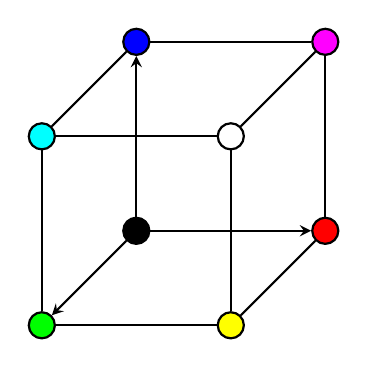
\begin{tikzpicture}
      \newcommand{\dist}[0]{24mm}
      \newcommand{\zdist}[0]{12mm}
      
      \tikzstyle{node}=[
        draw,
        circle,
        minimum height=0.2cm,
        minimum width=0.2cm,
        anchor=center,
        thick
      ]
      \tikzstyle{arrow} = [thick,->,>=stealth, draw=black]
      \tikzstyle{line} = [thick, draw=black]
      
      \definecolor{mycyan}{rgb}{0.0,1.0,1.0}
      \definecolor{mymagenta}{rgb}{1.0,0.0,1.0}
      \definecolor{myyellow}{rgb}{1.0,1.0,0.0}
      
      \node[node, fill=blue]      (blue)    at (0    , 0) {};
      \node[node, fill=mymagenta] (magenta) at (\dist, 0) {};
      \node[node, fill=black]     (black)   at (0    , -\dist) {};
      \node[node, fill=red]       (red)     at (\dist, -\dist) {};
      \node[node, fill=mycyan]   (cyan)   at (0-\zdist    , 0-\zdist) {};
      \node[node, fill=white]    (white)  at (\dist-\zdist, 0-\zdist) {};
      \node[node, fill=green]    (green)  at (0-\zdist    , -\dist-\zdist) {};
      \node[node, fill=myyellow] (yellow) at (\dist-\zdist, -\dist-\zdist) {};
      
      \draw[arrow] (black) -- (red);
      \draw[arrow] (black) -- (green);
      \draw[arrow] (black) -- (blue);
      \draw[line] (blue) -- (magenta);
      \draw[line] (blue) -- (cyan);
      \draw[line] (red) -- (magenta);
      \draw[line] (red) -- (yellow);
      \draw[line] (green) -- (yellow);
      \draw[line] (green) -- (cyan);
      \draw[line] (white) -- (cyan);
      \draw[line] (white) -- (magenta);
      \draw[line] (white) -- (yellow);
    \end{tikzpicture}
  }
\end{center}

  \caption{RGB color cube.}
  \label{fig:primdata:struct:color}
\end{figure}

% color spaces
This constitutes a \textsl{color space} whereby all colors fit within a color cube spanned by the red, green and blue color vectors. Hence, it is named the RGB color space. Figure \ref{fig:primdata:struct:color} depicts this space. It is a direct fit for how GPUs represent images. Other color spaces exist though, and there are good reasons for their existence. Other popular color spaces include HSV (which is shaped like a cylinder) and XYZ (which is shaped like an tongue). Formulas exists for converting between these. Each of these color spaces represents practical simplifications of what light really is.

\subsection{Points}

\section{Enumerations}

\subsection{State Machines}

\subsection{String Parsing Example}

